
\subsubsection{\stid{4.16} ALPINE} 


\paragraph{Overview} 

ECP ALPINE/{\zfp} will deliver in situ visualization and analysis infrastructure and algorithms along with lossy compression for floating point arrays to ECP Applications.  

\textbf{ALPINE} infrastructure developers come from the ParaView~\cite{alpine:Paraview1,alpine:Paraview2} and VisIt~\cite{alpine:VisIt} teams and ALPINE solutions will deliver in situ DAV functionality in those tools, as well as through Ascent~\cite{alpine:Ascent}, a new in situ infrastructure framework that focuses on flyweight processing. 
%
ALPINE  focuses on four major activities: 
\begin{enumerate}
        \setlength{\itemsep}{1pt}
        \setlength{\parskip}{0pt}
        \setlength{\parsep}{0pt}
\item Deliver Exascale visualization and analysis algorithms that will be critical for ECP Applications as the dominant analysis paradigm shifts from post hoc (post-processing) to in situ (processing data in a code as it is generated). 
\item Deliver an Exascale-capable infrastructure for the development of in situ algorithms and deployment into existing applications, libraries, and tools. 
\item Engage with ECP Applications to integrate our algorithms and infrastructure into their software. 
\item Engage with ECP Software Technologies to integrate their Exascale software into our infrastructure. 
\end{enumerate}


\paragraph{Key  Challenges}

Many high performance simulation codes are using post hoc processing.  
Given Exascale I/O and storage constraints, in situ processing will be necessary. 
In situ data analysis and visualization selects, analyzes, reduces, and generates extracts from scientific simulation results during the simulation runs to overcome bandwidth and storage bottlenecks associated with writing out full simulation results to disk. 
The ALPINE team is addressing two problems related to Exascale processing --- (1) delivering infrastructure and (2) delivering performant in situ algorithms.
The challenge for existing infrastructure tools is that need to become Exascale-ready in order to achieve performance within simulation codes’ time budgets, support many-core architectures, scale to massive concurrency, and leverage deep memory hierarchies. The challenge for in situ algorithms is to apply in situ processing effectively without a human being in the loop.
This means that we must have adaptive approaches to automate saving the correct visualizations and data extracts.


\paragraph{Solution Strategy}

A major strategy for our team is to leverage existing, successful software, ParaView and its in situ Catalyst~\cite{Catalyst} library and VisIt, and then to integrate and augment them with ALPINE data and analysis capabilities to address the challenges of Exascale. 
%
Both software projects represent long-term DOE investments, and they are the two dominant software packages for large-scale visualization and analysis within the DOE SC and the DOE NNSA. 
%These two products provide significant coverage of ECP Applications, and we can leverage their existing engagements to deliver ALPINE's algorithms and infrastructure. 
%Our development strategy consists of placing all new algorithms developed in a single code repository, and deploying this code in both
%ParaView and VisIt.
%
Our team is also developing an additional  in situ framework, Ascent.  Ascent is a ``flyweight'' solution, meaning that it is focused on a streamlined API, minimal memory footprint, and small binary size.
Our solution strategy is two-fold, in response to our two major challenges: infrastructure and algorithms.

For infrastructure, we have developed a layer on top of the VTK-m library for ALPINE algorithms.
This layer is where all ALPINE algorithms will be implemented, and it is deployed in ParaView/Catalyst, VisIt, and Ascent.
Thus all development effort by ALPINE will be available in all of our tools and by leveraging VTK-m, we will be addressing issues with many-core architectures.  
%Figure~\ref{fig:alpine_infrastructure} illustrates our software strategy.

%\begin{figure}[htb]
%	\centering
%	\includegraphics[width=3in]{projects/2.3.4-DataViz/2.3.4.16-ALPINE-ZFP/alpine_infrastructure.png}
%	\caption{\label{fig:alpine_infrastructure}ALPINE's strategy for delivering and developing software.  We are making use of existing software (ParaView, VisIt), but making sure all new development is shared in all of our tools.  The dotted lines represent ongoing work, specifically that the Ascent API will work with ParaView and VisIt.}
%\end{figure}

ALPINE is developing a suite of in situ  algorithms designed to address I/O and data output constraints and enable scientific discovery.   These algorithms include:
\begin{description}  
	\setlength{\itemsep}{1pt}
    \setlength{\parskip}{0pt}
    \setlength{\parsep}{0pt}
	\item [Topological analysis] can be used to detect features in the data and adaptively steer visualizations with no human in the loop.  For example, contour trees can identify the most significant isosurfaces in complex simulations and then the resulting visualizations can use these isosurfaces~\cite{alpine:Carr:TVCG19}.
	\item [Adaptive sampling]  can be used to guide visualizations and extracts to the most important parts of the simulation, significantly reducing I/O~\cite{alpine:Biswas:ISAV18,alpine:Dutta:Entropy19,alpine:Liu:SC19poster}.  %Figure~\ref{fig:alpine-sampling-example} shows an adaptive sampling technique based on importance to preserve  features in the data  
	\item [Statistical feature detection] models data using distribution-based approaches and statistical similarity measures to identify and isolate features of interest~\cite{alpine:Dutta:PVIS17,alpine:Dutta:VIS15}. Significant data reduction is possible by only saving the statistical representations of the data.  Figure~\ref{fig:alpine-statistical-feature} illustrates the use of the statistical feature detection approach to identifying bubbles in situ in an MFiX-Exa simulation.  
	\item [Task-based feature extraction] uses segmented merge trees to encode a wide range of threshold based features.  An embedded domain specific language (EDSL) can describe algorithms using a  task graph abstraction~\cite{alpine:Landge:SC14,alpine:Petruzza:IPDPS18} and execute it using different runtimes (e.g., MPI, Charm++, Legion).
	\item [Optimal Viewpoint] Optimal Viewpoint metrics can be used to automate visualization decisions while running in situ. The initial algorithm implementation will choose the best camera placement for a scene, minimizing visualizations written to disk~\cite{alpine:Bonaventura:Entropy18,alpine:Marsaglia:UOtech20}.  
	\item [Lagrangian analysis] of vector flow allows more efficient and complete tracking of flow.  It can save vector field data with higher accuracy and less storage than the traditional approaches~\cite{alpine:Sane:EGPGV18,alpine:Sane:EGPGV19,alpine:Binyahib:LDAV19}.
%	\item [Moments-based pattern detection] can be used to find rotation-invariant patterns~\cite{alpine:Bujack:WSCG17,alpine:Yang:PR17,alpine:Wang:TopoVis17}. 
\end{description}

%\begin{figure*}[htb]
%	\begin{center}
%	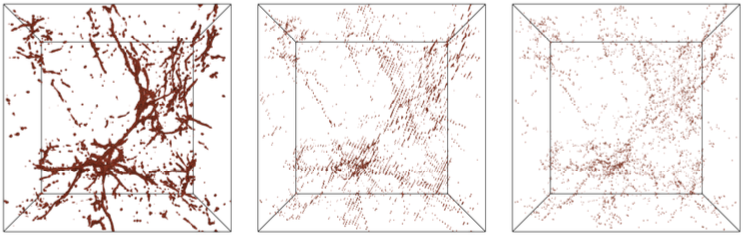
\includegraphics[width=0.65\textwidth]{projects/2.3.4-DataViz/2.3.4.16-ALPINE-ZFP/alpine_nyxSamplingExample.png}
%		\caption{Point rendering results from Nyx simulation using (left to right):  ALPINE adaptive sampling  (sampling ratio 0.5\%); regular sampling  (sampling ratio 1.5\%); random sampling  (sampling ratio 0.5\%).}
%		\label{fig:alpine-sampling-example}
%	\end{center}
%\end{figure*}

\paragraph{Recent Progress}

%During this past year, ALPINE has made considerable progress in core functionality in infrastructure and algorithms, and in creating a robust software stack to meet exascale data and viz needs.  ALPINE collaborated with the VTK-m team to port ALPINE functionality to early access systems.   
During this past year, ALPINE focused on porting infrastructure to early access systems; hardening algorithms by porting to VTK-m and ensuring comprehensive unit testing while furthering integrations with key clients.  ALPINE facility team members worked closely with the VTK-m team on porting activities such as builds on early access systems (EAS) and  HIP implementations. 

The ParaView/Catalyst team updated the build system to enable VTK-m with the CUDA back-end and tested on OLCF's Summit.  Likewise, the VisIt team deployed on Summit.  A  build of ParaView with minimal dependencies was also done on Spock.  Deployments included improvements to Spack build processes.   Team efforts also covered build and continuous integration activities for ALPINE infrastructure on NDA-restricted early access systems.   New VTK-m functionality such as distributed memory particle advection was deployed in Ascent.   Efforts are currently underway to deploy ALPINE infrastructure on Perlmutter.   

%ParaView utilized the Ascent python extract feature to add in situ visualization in Ascent via ParaView and redesigned the Catalyst in situ library for greater ease of use.  As more simulations have adapted in situ approaches, infrastructure integration has shifted from the domain of a small set of VTK-cognizant developers to application scientists who may not have experience with the VTK data model.  
%The new Catalyst adaptor leverages Ascent's Conduit API to describe data and provides schema to convert Conduit mesh descriptions to VTK data objects.  
%The initial design has been completed and prototyped.  

%New functionality in Ascent includes Jupyter notebook integration and new derived field quantities, enabling simulations instrumented with Ascent to connect to Jupyter and simulation users to interact with their data in situ using Jupyter Notebooks. 
%The Jupyter ecosystem of tools provides a rich paradigm for interactive data analysis. This work enables simulations instrumented with Ascent to connect to Jupyter and allows simulation users to interact with their data in situ using Jupyter Notebooks. 
%The system combines Ascent’s embedded Python filter infrastructure with a Client/Server Jupyter Bridge Kernel design that simplifies both deployment and security considerations on HPC systems. 
%Building on its existing query system, Ascent added a production-oriented in situ derived field system leveraging just-in-time (JIT) compilation to target heterogeneous HPC architectures.  Ascent's new derived quantities include topological functions, gradients, and basic math functions.  
%These new derived quantities were validated with an ECP application and with proxy apps within Ascent.  Additionally, a set of unit tests have been developed to exercise the derived quantities.   

% Algorithm improvements
Algorithms have  focused on hardening, deployment in VTK-m, and unit testing while integration with clients has continued.  With the sampling algorithm now fully GPU capable and the Ascent $<>$ ExaSky:Nyx integration in place, the sampling algorithm team has focused on post hoc reconstruction methods and support for AMR levels.

The Ascent $<>$ ExaLearn $<>$ Pele integration has made considerable progress by developing a full integration of ExaLearn's Genten, a Kokkos-based library for anomaly detection, Ascent and PeleLM.  This include updating the co-kurtosis filter in Ascent to directly access the Genten library.  In addition, the teams have maintained the PeleC pipeline with updated codes.  The joint effort is also exploring interesting science use cases for CombustionPele.

ALPINE and MFiX-Exa teams are collaborating on bubble finding with the statistical feature detection algorithm and a Catalyst integration.  The statistical feature algorithm has been deployed in VTK-m, verified with the Catalyst $<>$ MFiX-Exa pipeline and has been tested with over $54$ million particles per time step, running on NERSC's Cori.  Additional work has been done to support bubble tracking and data summarization techniques for further data reduction.  

%An initial C++ implementation of the statistical feature detection algorithm was integrated directly into the MFiX-Exa simulation to extract bubbles in situ with greater temporal resolution and a factor of 300 in data reduction.  A pipeline consisting of the in situ bubble extraction and post hoc Cinema workflow enables interactive exploration of bubble dynamics, Figure~\ref{fig:alpine-statistical-feature}.  The Kitware team recently finished the Catalyst integration into MFiX-Exa while the algorithm team finished an updated VTK-m version.  These are currently being merged for testing on Summit's GPU.  

%The contour tree algorithm recently completed an upgrade and VTK-m port for its distributed parallel version and will circle back to its integration with WarpX.   An Ascent $<->$ NekRS  integration has been demonstrated on Iris' CPUs and this effort is now looking at science use cases and in situ analysis needs.   ALPINE and ExaWind have recently prototyped an Ascent $<->$ AMR:Wind integration and the teams are assessing in situ analysis approaches.  

The contour tree algorithm was refactored to update to latest VTK-m functionality.   The team developed an OpenMP+MPI prototype to compute derived metrics based on a distributed contour tree representation.  These importance metrics are needed to identify important features found by this topological approach.  Additional regression and consistency tests were added as the algorithm has been hardened.  

ALPINE is developing a task-based feature detection approach that can be executed on non-MPI runtimes such as Charm++.  The task-based feature detection team made significant progress this year, developing the LegoFlow extension which enables composable patterns, making it easier to construct larger task graphs.   They enabled a LegoFlow-based pipeline for image compositing as well as parallel merge tree computation, testing with PeleLM and developed a workflow for relevance field computation.

% legoflow.png information:
%LegoFlow provides flexibility to construct complex dataflow graphs for in situ data analysis and visualization needs
%Extends Ascent to provide portable communication layer on top of non-MPI runtimes, e.g., Charm++
%Novel analytics implemented in LegoFlow, e.g., localized feature detection (relevance)

The optimal viewpoint team also made significant strides, parallelizing the algorithm, exploring optimal viewpoint metrics, developing search methods, and studying the temporal characteristics of optimal viewpoint metrics.  They ran a user evaluation study to identify the metrics most correlated with human preference.  An entropy-based metric was found to be most highly correlated and was used in the development and optimization of the optimal viewpoint over time (OVPOT) algorithm.  

\begin{figure*}[htb]
	\begin{center}
		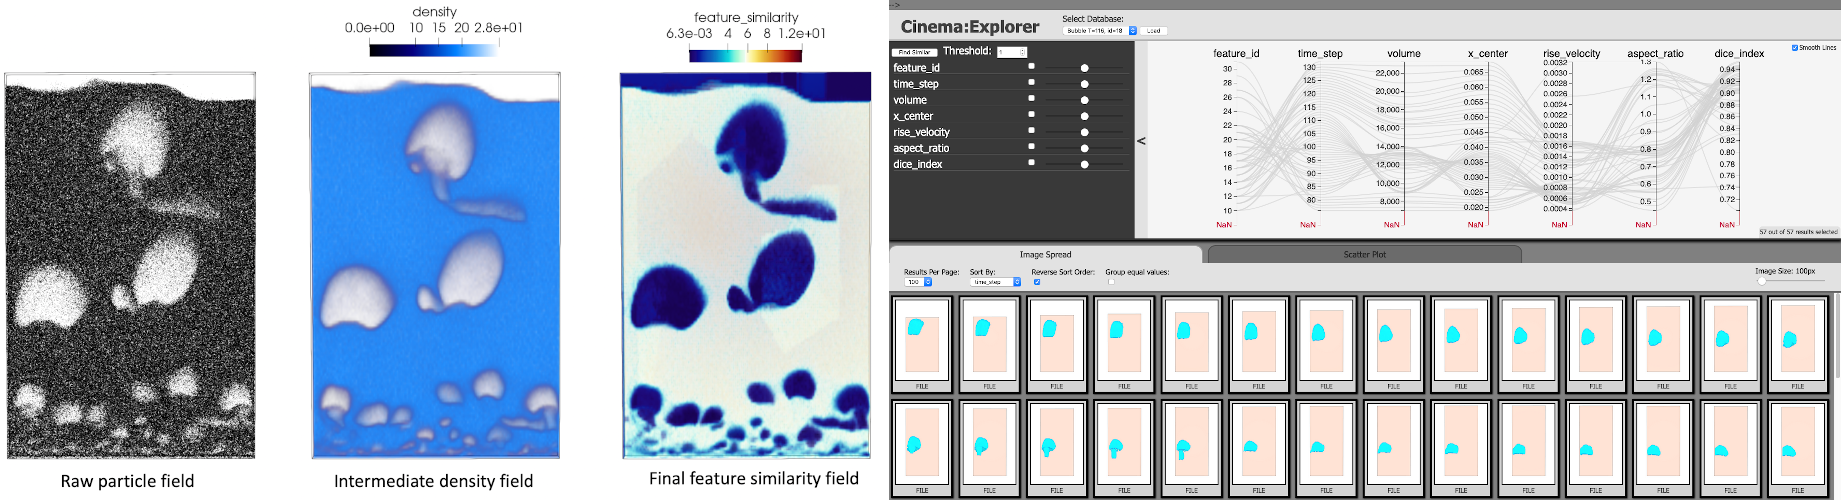
\includegraphics[width=0.95\textwidth]{projects/2.3.4-DataViz/2.3.4.16-ALPINE-ZFP/alpine-cinema-mfixexa-workflow.png}
		\caption{The ALPINE statistical feature detection algorithm is used to identify bubbles in situ in an MFiX-Exa fluidized bed simulation.  The raw article data is converted to a particle density field.  A threshold is applied to the density field to create a feature similarity field, separating the  bubbles from uninteresting regions.  Saving only the statistical representation allows greater temporal resolution while significantly reducing output data size.  A preliminary study shows a factor of 300 reduction in data size compared to the raw particle fields. The statistical bubble representation becomes the input to a post hoc Cinema-based workflow to track bubbles and explore bubble dynamics. }
		\label{fig:alpine-statistical-feature}
	\end{center}
\end{figure*}

\paragraph{Next Steps}

Plans for FY22-23 will continue the focus on integration and delivery to ECP applications.  This will include deploying key infrastructure and integration pipelines on Frontier. The team will also continue outreach with ECP application codes to support ECP applications codes as they shift their focus from  KPP-1 or KPP-2 runs to science runs and visualization needs.  

